\documentclass[aspectratio=1610]{beamer}
\usetheme{bjeldbak}
\usepackage{xspace}
\usepackage{graphicx}
\usepackage{textpos}
\usepackage{subfigure}
\usepackage{pifont}
\usepackage[super]{nth}
\usepackage{relsize}
\usepackage{amsmath}

\setbeamertemplate{section page}{
  \begin{centering}
    \begin{beamercolorbox}[sep=12pt,center]{part title}
      \huge
      \insertsection
    \end{beamercolorbox}
  \end{centering}
}

\definecolor{anti-flashwhite}{rgb}{0.95, 0.95, 0.96}

\setbeamercolor{section in toc}{fg=anti-flashwhite}

\setbeamertemplate{section page}{
  \begin{centering}
    \begin{beamercolorbox}[sep=12pt,center]{part title}
      \huge
      \insertsection
    \end{beamercolorbox}
  \end{centering}
}

\usepackage{ifthen}
\usepackage{mciteplus} 
\newboolean{uprightparticles}
\setboolean{uprightparticles}{false} %Set true for upright particle symbols
\usepackage{xspace} 
\usepackage{upgreek}

\input{lhcb-symbols-def}
\input{spd-symbols-def}
\input{tracking-symbols-def}

\def \Cseven {\ensuremath{\mathcal{C}_{7}^{(\ensuremath{\prime})}}\xspace}
\def \Cnine {\ensuremath{\mathcal{C}_{9}^{(\ensuremath{\prime})}}\xspace}
\def \Cten {\ensuremath{\mathcal{C}_{10}^{(\ensuremath{\prime})}}\xspace}
\def \Cnineten {\ensuremath{\mathcal{C}_{9,10}^{(\ensuremath{\prime})}}\xspace}

\usepackage{appendixnumberbeamer}
\expandafter\def\expandafter\insertshorttitle\expandafter{%
  \insertshorttitle\hfill\insertframenumber\,/\,\inserttotalframenumber}

\usepackage[linewidth=1pt]{mdframed}
\newenvironment{myenv}[1]
{\mdfsetup{
  frametitle={\colorbox{white}{\space#1\space}},
  innertopmargin=3pt,
  frametitleaboveskip=-\ht\strutbox,
  frametitlealignment=\center
}
\begin{mdframed}%
}
{\end{mdframed}}

\setbeamertemplate{blocks}[rounded][shadow=false]
\setbeamercolor{block body}{bg=barcolor!40,fg=black}
\setbeamercolor{block title}{bg=barcolor!20,fg=black}

\usepackage{tikz}
\usetikzlibrary{shapes,arrows}

\definecolor{babyblue}{rgb}{0.54, 0.81, 0.94}
\definecolor{byzantine}{rgb}{0.74, 0.2, 0.64}
\definecolor{anti-flashwhite}{rgb}{0.95, 0.95, 0.96}
\definecolor{burgundy}{rgb}{0.5, 0.0, 0.13}
\definecolor{burntorange}{rgb}{0.8, 0.33, 0.0}
\definecolor{cadmiumorange}{rgb}{0.93, 0.53, 0.18}
\definecolor{bleudefrance}{rgb}{0.19, 0.55, 0.91}
\definecolor{bostonuniversityred}{rgb}{0.8, 0.0, 0.0}
\definecolor{darkred}{rgb}{0.55, 0.0, 0.0}
\definecolor{blue(ryb)}{rgb}{0.01, 0.28, 1.0}
\definecolor{darkgreen}{rgb}{0.0, 0.5, 0.0}
\definecolor{palatinatepurple}{rgb}{0.41, 0.16, 0.38}
\definecolor{cadmiumorange}{rgb}{0.93, 0.53, 0.18}
\definecolor{ceruleanblue}{rgb}{0.16, 0.32, 0.75}

%%%%%%%%%%%%%%%%%%%%%%%%%%%%%%%%%%%%%%%%%%%%%%%%%%%%%%%%%%%%%%%%%
%Begin document
%%%%%%%%%%%%%%%%%%%%%%%%%%%%%%%%%%%%%%%%%%%%%%%%%%%%%%%%%%%%%%%%%
\begin{document}
\title[]{Upstream Tracking and the Decay $\B^{0} \to K^{+}\pi^{-}\mu^{+}\mu^{-}$\\ at the LHCb Experiment}
\author[Espen Eie Bowen]{{\bf Espen Eie Bowen} \\ {\small PhD defense presentation}} 
\institute[]{}
\date{\nth{19} January 2017}
%%%%%%%%%%%%%%%%%%%%%%%%%%%%%%%%%%%%%%%%%%%%%%%%%%%%%%%%%%%%%%%%%
%Title
%%%%%%%%%%%%%%%%%%%%%%%%%%%%%%%%%%%%%%%%%%%%%%%%%%%%%%%%%%%%%%%%%
\begin{frame}[plain]
\titlepage
\begin{textblock*}{2cm}(12.5cm,0.0cm)
  \includegraphics[width=2cm]{figs/lhcb-logo.pdf}
\end{textblock*}
\begin{textblock*}{5cm}(0.0cm,0.0cm)
  \includegraphics[width=3.0cm]{figs/uzh.jpg}
\end{textblock*}
\end{frame}

%%%%%%%%%%%%%%%%%%%%%%%%%%%%%%%%%%%%%%%%%%%%%%%%%%%%%%%%%%%%%%%%%
%Slide
%%%%%%%%%%%%%%%%%%%%%%%%%%%%%%%%%%%%%%%%%%%%%%%%%%%%%%%%%%%%%%%%%
\begin{frame}{The \lhcb experiment}
  \begin{itemize}
  \item LHCb is the dedicated heavy flavour physics experiment at the LHC
  \item Its primary goal is to look for indirect evidence of new physics in CP violation and rare decays of beauty and charm hadrons
  \item This requires:
    \begin{enumerate}
    \item Excellent tracking 
      \begin{itemize}
      \item momentum resolution($\delta p/p \sim 0.4\% - 0.6\%$)
      \item impact parameter resolution ($\sigma_{IP} \sim 20~\mu$m)
      \item primary vertex resolution (13 $\mu$m in $x$ and $y$ and 71 $\mu$m in $z$)
      \end{itemize}
    \item Excellent decay time resolution ($\sigma_{\tau}$ $\sim$ 45~fs)
    \item Excellent particle identification
    \end{enumerate}
  \end{itemize}

    \bigskip
    
    \begin{columns}
      \begin{column}{0.29\textwidth}
        \centering
        \begin{tikzpicture}
          \node[anchor=south west,inner sep=0] at (0,0) {\includegraphics[height=3.5cm]{figs/lhcb/massres.pdf}};
          \node[draw=none,barcolor!80!black] at (1.4,0.15) {\tiny \href{http://link.springer.com/article/10.1007\%2FJHEP06(2013)064}{JHEP 06 (2013) 064}};
        \end{tikzpicture}
      \end{column}
      \begin{column}{0.36\textwidth}
        \centering
        \begin{tikzpicture}
          \node[anchor=south west,inner sep=0] at (0,0) {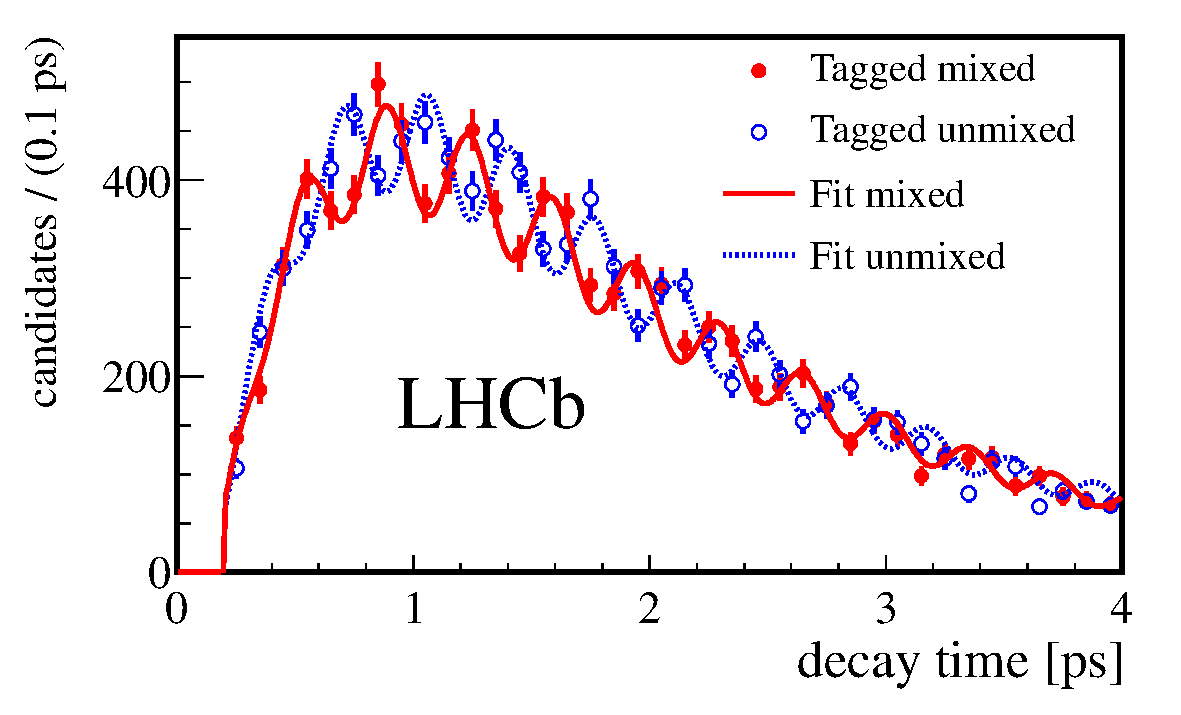
\includegraphics[height=3.5cm]{figs/lhcb/bsmix.pdf}};
          \node[draw=none,barcolor!80!black] at (2.2,0.15) {\tiny \href{http://iopscience.iop.org/1367-2630/15/5/053021/}{New~J.~Phys. 15 (2013) 053021}};
        \end{tikzpicture}
      \end{column}
      \begin{column}{0.36\textwidth}
        \begin{tikzpicture}
          \node[anchor=south west,inner sep=0] at (0,0) {\includegraphics[height=3.5cm]{figs/lhcb/RICH.png}};
          \node[draw=none,barcolor!80!black] at (1.4,0.15) {\tiny \href{http://epjc.epj.org/articles/epjc/abs/2013/05/10052_2013_Article_2431/10052_2013_Article_2431.html}{Eur. Phys. J. C (2013) 73}};
          \end{tikzpicture}
      \end{column}
    \end{columns}
\end{frame}

%%%%%%%%%%%%%%%%%%%%%%%%%%%%%%%%%%%%%%%%%%%%%%%%%%%%%%%%%%%%%%%%%
%Slide
%%%%%%%%%%%%%%%%%%%%%%%%%%%%%%%%%%%%%%%%%%%%%%%%%%%%%%%%%%%%%%%%%
\begin{frame}\frametitle{}
  \begin{center}
    \begin{tikzpicture}
      \node[anchor=south west,inner sep=0](image) at (0,0) {\includegraphics[width=\textwidth]{figs/lhcb/lhcb2.png}};
      
      \begin{scope}[x={(image.south east)},y={(image.north west)}]
        %\draw[help lines,xstep=.1,ystep=.1] (0,0) grid (1,1);
        
        \node[draw=none,burgundy] at (0.15,0.05) {Vertex Locator};
        \draw[ultra thick,->,burgundy] (0.15,0.1) -- (0.2,0.4);
        
        \node[draw=none,cadmiumorange] at (0.18,0.95) {Tracking system (TT,IT,OT)};
        \draw[ultra thick,->,cadmiumorange] (0.1,0.9) -- (0.3,0.48);
        \draw[ultra thick,->,cadmiumorange] (0.1,0.9) -- (0.58,0.52); 
        
        \node[draw=none,byzantine] at (0.48,0.95) {Rich detectors};
        \draw[ultra thick,->,byzantine] (0.5,0.9) -- (0.23,0.55);
        \draw[ultra thick,->,byzantine] (0.5,0.9) -- (0.65,0.65);
        
        \node[draw=none,gray] at (0.45,0.2) {Magnet};
        
        \node[draw=none,babyblue] at (0.7,0.05) {Calorimeters};
        \draw[ultra thick,->,babyblue] (0.7,0.1) -- (0.75,0.55);
        
        \node[draw=none,green!90!black] at (0.9,0.7) {Muon system};
        
      \end{scope}
    \end{tikzpicture}
    
  \end{center}
\end{frame}

%%%%%%%%%%%%%%%%%%%%%%%%%%%%%%%%%%%%%%%%%%%%%%%%%%%%%%%%%%%%%%%%%
%Slide
%%%%%%%%%%%%%%%%%%%%%%%%%%%%%%%%%%%%%%%%%%%%%%%%%%%%%%%%%%%%%%%%%
\begin{frame}{Track reconstruction at \lhcb}

\end{frame}

%%%%%%%%%%%%%%%%%%%%%%%%%%%%%%%%%%%%%%%%%%%%%%%%%%%%%%%%%%%%%%%%%
%Slide
%%%%%%%%%%%%%%%%%%%%%%%%%%%%%%%%%%%%%%%%%%%%%%%%%%%%%%%%%%%%%%%%%
\begin{frame}\frametitle{Upstream tracking in Run 1}
  \begin{itemize}
  \item Linearly extrapolate VELO track to TT
  \item Open search windows in each layer and find $\Delta x$ between track and hits
  \item Scale $\Delta x$ to reference plane at center of TT
  \item Choose clusters of hits consistent with coming from the same VELO track
  \begin{itemize}
    \item[\ding{72}] Each hit must be on the same side of the linear extrapolation
  \end{itemize}
  \item Fit each track candidate with a simple $\chi^{2}$ fit
  \item Choose best candidate track based on \# layers fired and $\chi^{2}$
  \item Fit track with \underline{full Kalman filter}
  \end{itemize}
  \input{figs/tikz/tracking-velott}
\end{frame}

%%%%%%%%%%%%%%%%%%%%%%%%%%%%%%%%%%%%%%%%%%%%%%%%%%%%%%%%%%%%%%%%%
%Slide
%%%%%%%%%%%%%%%%%%%%%%%%%%%%%%%%%%%%%%%%%%%%%%%%%%%%%%%%%%%%%%%%%
\begin{frame}{Novel idea: Upstream tracking for the Upgrade}
\begin{itemize}
  \item Upstream tracks could the speed up the tracking sequence of the Upgrade software trigger
  \item Advantages over using VELO tracks
    \begin{itemize}
      \item Charge and momentum of track segment ($\delta \ptot/\ptot \sim 15 \%$)
      \begin{itemize}
        \item[\ding{212}] Preselect on track \pt
        \item[\ding{212}] Open smaller search windows
        \item[\ding{72}] Greatly reduce execution time and ghost rate!
      \end{itemize}
    \end{itemize}
  \end{itemize}

  \begin{center}
  \input{figs/tikz/upstream-tracking-upgrade-search-window}
  \end{center}

  \begin{itemize}
  \item Upstream tracking algorithm needs to be optimised for speed/efficiency
  \end{itemize}
\end{frame}

%%%%%%%%%%%%%%%%%%%%%%%%%%%%%%%%%%%%%%%%%%%%%%%%%%%%%%%%%%%%%%%%%
%Slide
%%%%%%%%%%%%%%%%%%%%%%%%%%%%%%%%%%%%%%%%%%%%%%%%%%%%%%%%%%%%%%%%%
\begin{frame}{VeloUT: Initial peformance}

\begin{columns}
\begin{column}{0.65\textwidth}
\resizebox{1.0\textwidth}{!}{
\begin{tabular}{c|c|c|c}
\velout & Efficiency [\%] & Ghost rate [\%] & Timing [ms] \\ 
\hline
v1r2  & 93.94  & 7.21  &  27.20  \\ 
\end{tabular}
}
\end{column}
\begin{column}{0.35\textwidth}
\centering
\begin{figure}
\vspace*{-1cm}
\includegraphics[height=0.475\textheight]{figs/upstream-tracking-upgrade/eff_p_v1r2.pdf}\\
\includegraphics[height=0.475\textheight]{figs/upstream-tracking-upgrade/gr_p_v1r2.pdf}
\end{figure}
\end{column}
\end{columns}

\end{frame}

%%%%%%%%%%%%%%%%%%%%%%%%%%%%%%%%%%%%%%%%%%%%%%%%%%%%%%%%%%%%%%%%%
%Slide
%%%%%%%%%%%%%%%%%%%%%%%%%%%%%%%%%%%%%%%%%%%%%%%%%%%%%%%%%%%%%%%%%
\begin{frame}{Optimised upstream algorithm}
\begin{columns}
\begin{column}{0.5\textwidth}
\begin{itemize}
  \item[$\blacktriangleright$] Linearly extrapolate VELO track to TT
  \item[\ding{72}] Select hits within a search window around the extrapolated track
  \item[\ding{72}] Form doublets of hits in the first two layers
  \item[\ding{72}] Extrapolate doublets to third/fourth layers and search for compatible hits
  \item[\ding{72}] If no four hit candidates found, repeat in starting from last two layers
  \item[$\blacktriangleright$] Fit each track candidate with a $\chi^{2}$ fit and estimate $q/p$ ($\delta p/p \sim 15 \%$)
  \item[$\blacktriangleright$] Choose best candidate track based on \# layers fired and $\chi^{2}$
  \end{itemize}
\end{column}
\begin{column}{0.5\textwidth}
\centering
\input{figs/tikz/upstream-tracking-upgrade-clustering}
\end{column}
\end{columns}
\end{frame}

%%%%%%%%%%%%%%%%%%%%%%%%%%%%%%%%%%%%%%%%%%%%%%%%%%%%%%%%%%%%%%%%%
%Slide
%%%%%%%%%%%%%%%%%%%%%%%%%%%%%%%%%%%%%%%%%%%%%%%%%%%%%%%%%%%%%%%%%
\begin{frame}{VeloUT: Optimised peformance}

\begin{columns}
\begin{column}{0.65\textwidth}
\resizebox{1.0\textwidth}{!}{
\begin{tabular}{c|c|c|c}
\velout & Efficiency [\%] & Ghost rate [\%] & Timing [ms] \\ 
\hline
v1r2  & 93.94  & 7.21  &  27.20  \\
v2r2  & 98.69  & 8.00 &  \hphantom{0}0.81  \\
\end{tabular}
}
\end{column}
\begin{column}{0.35\textwidth}
\centering
\begin{figure}
\vspace*{-1cm}
\includegraphics[height=0.475\textheight]{figs/upstream-tracking-upgrade/eff_p_comp.pdf}\\
\includegraphics[height=0.475\textheight]{figs/upstream-tracking-upgrade/gr_p_comp.pdf}
\end{figure}
\end{column}
\end{columns}

\end{frame}

%%%%%%%%%%%%%%%%%%%%%%%%%%%%%%%%%%%%%%%%%%%%%%%%%%%%%%%%%%%%%%%%%
%Slide
%%%%%%%%%%%%%%%%%%%%%%%%%%%%%%%%%%%%%%%%%%%%%%%%%%%%%%%%%%%%%%%%%
\begin{frame}{\BdToKpimm}

\end{frame}

%%%%%%%%%%%%%%%%%%%%%%%%%%%%%%%%%%%%%%%%%%%%%%%%%%%%%%%%%%%%%%%%%
%Backup
%%%%%%%%%%%%%%%%%%%%%%%%%%%%%%%%%%%%%%%%%%%%%%%%%%%%%%%%%%%%%%%%%
\appendix

%%%%%%%%%%%%%%%%%%%%%%%%%%%%%%%%%%%%%%%%%%%%%%%%%%%%%%%%%%%%%%%%%
%Slide
%%%%%%%%%%%%%%%%%%%%%%%%%%%%%%%%%%%%%%%%%%%%%%%%%%%%%%%%%%%%%%%%%
\begin{frame}[plain]
\centering 
\Huge Backup slides
\end{frame}

%%%%%%%%%%%%%%%%%%%%%%%%%%%%%%%%%%%%%%%%%%%%%%%%%%%%%%%%%%%%%%%%%
%Slide
%%%%%%%%%%%%%%%%%%%%%%%%%%%%%%%%%%%%%%%%%%%%%%%%%%%%%%%%%%%%%%%%%
\begin{frame}{}

\end{frame}

%%%%%%%%%%%%%%%%%%%%%%%%%%%%%%%%%%%%%%%%%%%%%%%%%%%%%%%%%%%%%%%%%%%%%%%%%%%%%%%%%%%%%%%
%%%%%%%%%%%%%%%%%%%%%%%%%%%%%%%%%%%%%%%%%%%%%%%%%%%%%%%%%%%%%%%%%%%%%%%%%%%%%%%%%%%%%%%
%           END OF DOCUMENT
%%%%%%%%%%%%%%%%%%%%%%%%%%%%%%%%%%%%%%%%%%%%%%%%%%%%%%%%%%%%%%%%%%%%%%%%%%%%%%%%%%%%%%%
%%%%%%%%%%%%%%%%%%%%%%%%%%%%%%%%%%%%%%%%%%%%%%%%%%%%%%%%%%%%%%%%%%%%%%%%%%%%%%%%%%%%%%%
\end{document}


